\documentclass{assignment}
\UsingEnglish
\ProjectInfos*{Introduction to System System}{EE140}{Fall, 2020}{Assignment 3}{Due time : 10:15, Oct 9, 2020 (Friday)}{陈稼霖}{45875852}
\begin{document}
\begin{prob}[Autocorrelation and cross-correlation function, 30 pts]
    The random process are given by $X(t)=n(t)+A\cos(2\pi f_0t+\theta)$, $Y(t)=n(t)+A\sin(2\pi f_0t+\theta)$, where $A$ and $f_0$ are positive constants and $\theta$ is a random variable uniformly distributed in the interval $[-\pi,\pi)$. The first term $n(t)$ represents a stationary random noise process with autocorrelation function $R_n(\tau)=B\Lambda(\tau)+C$, where $B$ and $C$ are positive constants. We further assume the random process $n(t)$ and $A\cos(2\pi f_0t+\theta)$ are uncorrelated, $n(t)$ and $A\sin(2\pi f_0t+\theta)$ are also uncorrelated.
    \begin{itemize}
        \item[1)] Find the autocorrelation functions of $X(t)$ and $Y(t)$, respectively.
        \item[2)] Find the cross-correlation function of $X(t)$ and $Y(t)$.
        \item[3)] Find the power spectral densities of $X(t)$ and $Y(t)$, respectively.
        \item[4)] Find the cross power spectral density of $X(t)$ and $Y(t)$.
        \item[5)] Find the total power of $X(t)$ and $Y(t)$, respectively.
        \item[6)] Find the DC powers of $X(t)$ and $Y(t)$, respectively.
    \end{itemize}
    (Hint: $\Lambda(\tau)=\left\{\begin{array}{ll}
        1-\abs{\tau},&\abs{\tau}\leq 1\\
        0,&\text{otherwise}
    \end{array}\right.$, the DC power of $X(t)$ is $\overline{X(t)}^2=E^2[X(t)]$)
\end{prob}
\begin{sol}
    \begin{itemize}
        \item[1)] The autocorrelation function of $X(t)$ is
        \begin{align}
            \notag R_X(t,t+\tau)=&E[X(t)X(t+\tau)]=E\{[n(t)+A\cos(2\pi f_0t+\theta)][n(t+\tau)+A\cos(2\pi f_0(t+\tau)+\theta)]\}\\
            \notag=&E[n(t)n(t+\tau)]+E[n(t)A\cos(2\pi f_t(t+\tau)+\theta)]\\
            \notag&+E[A\cos(2\pi f_0t+\theta)n(t+\tau)]+E[A\cos(2\pi f_0t+\theta)A\cos(2\pi f_0(t+\tau)+\theta)]\\
            \notag&(\because n(t)\text{ and }A\cos(2\pi f_0t+\theta)\text{ are uncorrelated})\\
            \notag=&R_X(\tau)+E[n(t)]E[A\cos(2\pi f_0(t+\tau)+\theta)]\\
            \notag&+E[A\cos(2\pi f_0t+\theta)]E[n(t+\tau)]+A^2E[\cos(2\pi f_0t+\theta)\cos(2\pi f_0(t+\tau)+\theta)]\\
            \notag=&B\Lambda(\tau)+C+\frac{A^2}{2}\int_{-\pi}^{\pi}[\cos(4\pi f_0t+2\pi f_0\tau+2\theta)+\cos(2\pi f_0\tau)]\frac{1}{2\pi}\,d\theta\\
            =&B\Lambda(\tau)+C+\frac{A^2}{2}\cos(2\pi f_0\tau).
        \end{align}
        Similarly, the autocorrelation function of $Y(t)$ is
        \begin{align}
            \notag R_Y(t,t+\tau)=&E[Y(t)Y(t+\tau)]=E\{[n(t)+A\sin(2\pi f_0t+\theta)][n(t+\tau)+A\sin(2\pi f_0(t+\tau)+\theta)]\}\\
            \notag=&E[X(t)X(t+\tau)]+E[n(t)A\sin(2\pi f_0(t+\tau)+\theta)]\\
            \notag&+E[A\sin(2\pi f_0t+\theta)n(t+\tau)]+E[A\sin(2\pi f_0t+\theta)A\sin(2\pi f_0(t+\tau)+\theta)]\\
            \notag&(\because n(t)\text{ and }A\sin(2\pi f_0t+\theta)\text{ are uncorrelated})\\
            \notag=&R_n(\tau)+E[n(t)]E[A\sin(2\pi f_0t+\theta)]\\
            \notag&+E[A\sin(2\pi f_0t+\theta)]E[n(t+\tau)]+A^2E[\sin(2\pi f_0t+\theta)\sin(2\pi f_0(t+\tau)+\theta)]\\
            \notag=&B\Lambda(\tau)+C+\frac{A^2}{2}\int_{-\pi}^{\pi}[\cos(2\pi f_0t)-\cos(4\pi f_0t+2\pi f_0\tau+2\theta)]\frac{1}{2\pi}\,d\theta\\
            =&B\Lambda(\tau)+C+\frac{A^2}{2}\cos(2\pi f_0\tau).
        \end{align}
        \item[2)] The cross-correlation function of $X(t)$ and $Y(t)$ is
        \begin{align}
            \notag R_{X,Y}(t,\tau)=&E[X(t)Y(t+\tau)]=E\{[n(t)+A\cos(2\pi f_0t+\theta)][n(t+\tau)+A\sin(2\pi f_0(t+\tau)+\theta)]\}\\
            \notag=&E[n(t)n(t+\tau)]+E[n(t)A\sin(2\pi f_0(t+\tau)+\theta)]\\
            \notag+&E[A\cos(2\pi f_0t+\theta)n(t+\tau)]+E[A\cos(2\pi f_0t+\theta)A\sin(2\pi f_0(t+\tau)+\theta)]\\
            \notag&(\because n(t)\text{ and }A\cos(2\pi f_0t+\theta)\text{ are uncorrelated, }n(t)\text{ and }A\sin(2\pi f_0t+\theta)\text{ are uncorrelated})\\
            \notag=&R_n(\tau)+E[n(t)]E[A\sin(2\pi f_0(t+\tau)+\theta)]+E[A\cos(2\pi f_0t+\theta)]E[n(t+\tau)]\\
            \notag&+E[A\sin(2\pi f_0(t+\tau)+\theta)]+A^2E[\cos(2\pi f_0t+\theta)\sin(2\pi f_0(t+\tau)+\theta)]\\
            \notag=&B\Lambda(\tau)+C+\frac{A^2}{2}\int_{-\pi}^{\pi}[\sin(4\pi f_0t+2\pi f_0\tau+2\theta)+\sin(2\pi f_0\tau)]\frac{1}{2\pi}\,d\theta\\
            =&B\Lambda(\tau)+C+\frac{A^2}{2}\sin(2\pi f_0\tau).
        \end{align}
        \item[3)] The first-order statistics of $X(t)$
        \begin{align}
            E[X(t)]=&E[n(t)+A\cos(2\pi f_0t+\theta)]=E[n(t)]+AE[\cos(2\pi f_0t+\theta)]=0+0=0,\\
            E\{[X(t)-E[X(t)]]^2\}=&E[X^2(t)]-E^2[X(t)]=E[X^2(t)]=R_X(t,t)=B+C+\frac{A^2}{2},
        \end{align}
        are not dependent on $t$, and as obtained in 1), the second-order statistics of $X(t)$ only depends on the gap, so $X(t)$ is wide-sense stationary. According to Wiener-Khinchine, the power spectral density of $X(t)$ is
        \begin{align}
            \notag S_X(t)=&\mathscr{F}[R_X(\tau)]=\mathscr{F}\left[B\Lambda(\tau)+C+\frac{A^2}{2}\cos(2\pi f_0\tau)\right]\\
            =&B\sinc^2\left(\frac{f}{2}\right)+C\delta(f)+\frac{A^2}{4}\left[\delta(f-f_0)+\delta(f+f_0)\right].
        \end{align}
        Similarly, the first-order statistics of $Y(t)$
        \begin{align}
            E[Y(t)]=&E[n(t)+A\sin(2\pi f_0t+\theta)]=E[n(t)]+AE[\sin(2\pi f_0t+\theta)]=0+0=0,\\
            E\{[Y(t)-E[Y(t)]]^2\}=&E[Y^2(t)]-E^2[Y(t)]=E[Y^2(t)]=R_Y(t,t)=B+C+\frac{A^2}{2},
        \end{align}
        are not dependent on $t$, and as obtained in 2), the second-order statistics of $Y(t)$ only depends on the gap, so $Y(t)$ is wide-sense stationary. According to Wiener-Khinchine theorem, the power spectral density of $Y(t)$ is
        \begin{align}
            \notag S_Y(t)=&\mathscr{F}[R_Y(\tau)]=\mathscr{F}\left[B\Lambda(\tau)+C+\frac{A^2}{2}\cos(2\pi f_0\tau)\right]\\
            =&B\sinc^2\left(\frac{f}{2}\right)+C\delta(f)+\frac{A^2}{4}\left[\delta(f-f_0)+\delta(f+f_0)\right].
        \end{align}
        \item[4)] As we obtained in 3), both $X(t)$ and $Y(t)$ are wide-sense stationary. The cross power of $X(t)$ and $Y(t)$ is
        \begin{align}
            \notag S_{XY}(f)=&\mathscr{F}[R_{XY}(\tau)]=\mathscr{F}\left[B\Lambda(\tau)+C+\frac{A^2}{2}\sin(2\pi f_0\tau)\right]\\
            =&B\sinc^2\left(\frac{f}{2}\right)+C\delta(f)+\frac{A^2}{4j}\left[\delta(f-f_0)-\delta(f+f_0)\right].
        \end{align}
        \item[5)] The total power of $X(t)$ is
        \begin{align}
            P_X=E[X^2(t)]=R_X(\tau=0)=B+C+\frac{A^2}{2}.
        \end{align}
        Similarly, the total power of $Y(t)$ is
        \begin{align}
            P_Y=E[Y^2(t)]=R_Y(\tau=0)=B+C+\frac{A^2}{2}.
        \end{align}
        \item[6)] Since the total power of $X(t)$ is a constant, the DC power of $X(t)$ is
        \begin{align}
            P_{X,\text{DC}}=P_X=B+C+\frac{A^2}{2}.
        \end{align}
        Similarly, since the total power of $Y(t)$ is a constant, the DC power of $Y(t)$ is
        \begin{align}
            P_{Y,\text{DC}}=P_Y=B+C+\frac{A^2}{2}.
        \end{align}
    \end{itemize}
\end{sol}

\begin{prob}[Gaussian random process transmission through a linear system, 30 pts]
    The input to a lowpass filter with impulse response $h(t)=\exp(-10t)u(t)$ is white, Gaussian noise with two-sided power spectral density of $2$W/Hz. Obtain the following:
    \begin{itemize}
        \item[1)] The mean of the output.
        \item[2)] The power spectral density of the output.
        \item[3)] The autocorrelation function of the output.
        \item[4)] The probability density function of the output at an arbitrary time $t_1$.
        \item[5)] The joint probability density function of the output at times $t_1$ and $t_1+2$.
        \item[6)] Find the noise equivalent bandwidth of the filter.
    \end{itemize}
    (Hint: $\mathscr{F}[\exp(-\alpha t)u(t),\alpha>0]=\frac{1}{\alpha+j2\pi f}$, $\mathscr{F}[\exp(-\alpha\abs{t}),\alpha>0]=\frac{2\alpha}{\alpha^2+(2\pi f)^2}$)
\end{prob}
\begin{sol}
    
\end{sol}

\begin{prob}[Narrowband noise, 40pts]
    Noise $n(t)$ has the power spectral density shown in the figure \ref{figure1}. We write $n(t)=n_c(t)\cos(2\pi f_0t+\theta)-n_s(t)\sin(2\pi f_0t+\theta)$, find and plot $S_{n_c}(f)$, $S_{n_s}(f)$ and $S_{n_cn_s}(f)$ fot the following case.
    \begin{itemize}
        \item[1)] $f_0=f_1$
        \item[2)] $f_0=f_2$
        \item[3)] $f_0=(f_1+f_2)/2$
        \item[4)] For which of these cases are $n_c(t)$ and $n_s(t)$ uncorrelated.
    \end{itemize}
    \begin{figure}[h]
        \centering
        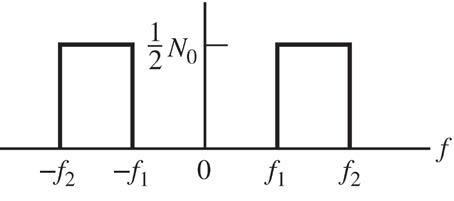
\includegraphics[width=.5\textwidth]{Figure1.jpg}
        \caption{$S_n(f)$}\label{figure1}
    \end{figure}
\end{prob}
\begin{sol}
    
\end{sol}
\end{document}